\documentclass{article}
\usepackage[utf8]{inputenc}
\usepackage{amsmath}
\usepackage{amsfonts}
\usepackage{mathrsfs}
\usepackage{graphicx}
\usepackage[top=30truemm,bottom=30truemm,left=30truemm,right=30truemm]{geometry}


\title{Chaotic Dynamics: Homework 3}
\author{Kansuke Ikehara (Kansuke.Ikehara@colorado.edu)}

\begin{document}
\maketitle

\subsection*{Problem 0}
\begin{figure}[hb]
	\centering
	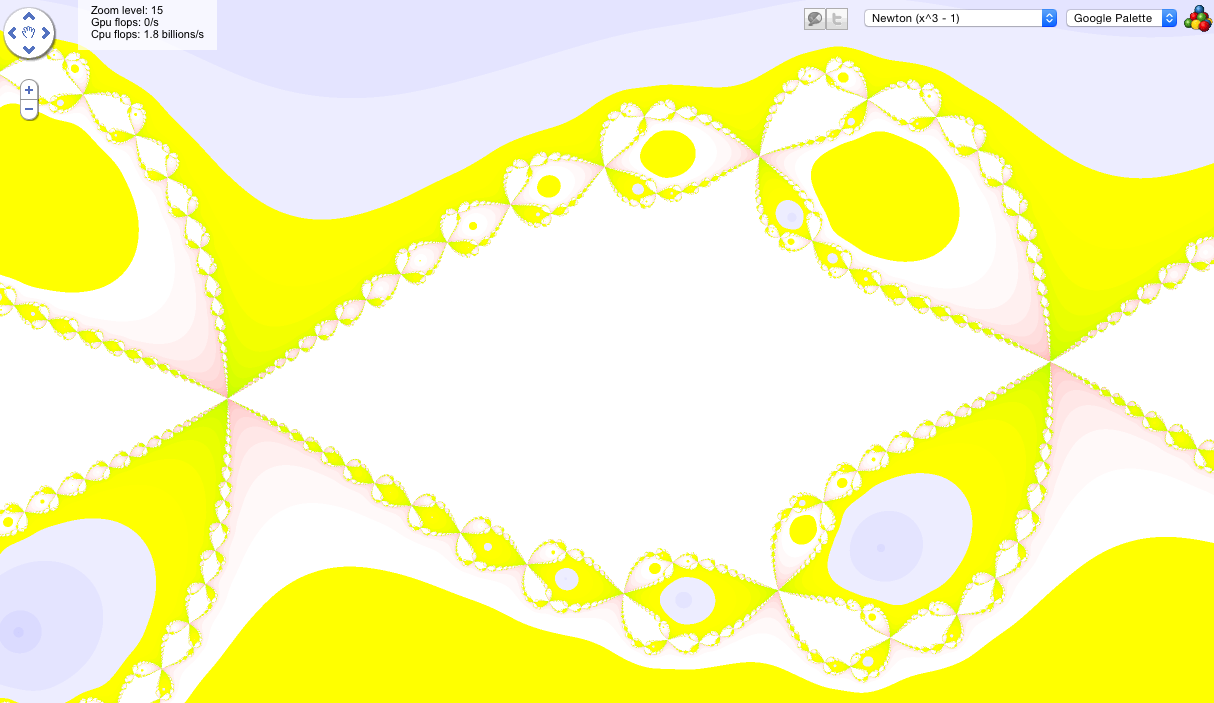
\includegraphics[height=2in]{figs/screen_shot.png}
	\caption{a screen shot of Newton's method}
	\label{screen_shot}
\end{figure}
Fig.\ref{screen_shot} shows an area of the plot of Newton's method that I find interesting and beautiful.

\subsection*{Problem 1}
After $k$ iterations of creating a middle-sixth-removed Cantor set, we have $N(\epsilon)$ and $\epsilon$ as follows:
\[
	N(\epsilon) = 2^{k}, \epsilon = \left( \frac{2.5}{6} \right)^k
\]
So in the limit of $k  \to \infty$, the capacity dimension of the set is:
\[
	d_{cap} = \lim_{k  \to \infty}\frac{\log(2^k)}{\log\left( \frac{6}{2.5} \right)^k} = \frac{\log2}{\log\left( \frac{6}{2.5} \right)} \approx 0.79
\]

\subsection*{Problem 2}
\subsubsection*{(a)}
After 4 steps as explained in \textit{ODE notes}, we have the following three first-order ODEs:
\[
	\dot{x} = y
\]
\[
	\dot{y} = z
\]
\[
	\dot{z} = \frac{3}{2}\tan\left( \frac{1}{2}z\right) -8\log(y) + \frac{1}{2}x
\]
\subsubsection*{(b)}
By substituting equations back and forth, we have the following single third-order ODE:
\[
	\dddot{x} = \ddot{x}\dot{x} + \log{\dot{x}}
\]
\subsubsection*{(c)}
For (a), the terms $\tan\left( \frac{1}{2}z\right)$ and $\log(y)$ are non-linear, thus the system is non-linear as well. For (b), the terms $yz$ and $\log(y)$ are non-linear, thus the system is non-linear.

\subsection*{Problem 3}
\subsubsection*{(a)}
\begin{figure}[hb]
	\centering
	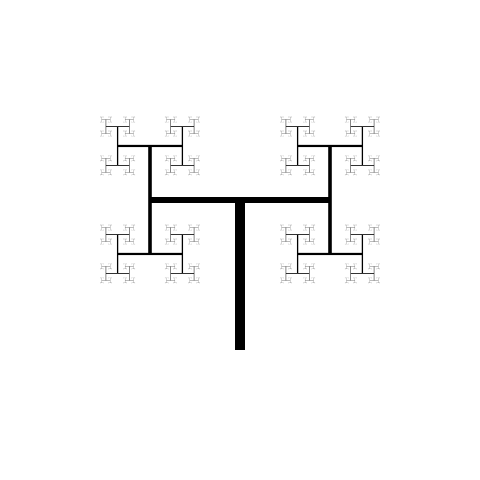
\includegraphics[height=3in]{figs/fractal-tree_06.png}
	\caption{a fractal tree with the length ratio of $0.6$ and $90$ degree.}
	\label{fractal_tree1}
\end{figure}

Fig.\ref{fractal_tree1} shows a fractal tree with the length ratio of $0.6$ and $90$ degree for both left and right branches. The capacity dimension of such a tree can be calculated as follows: as we go the tree deeper and deeper, the number of \textit{boxes} needed to cover leaves grows as $2^k$, where $k$ is the depth of the tree, and the size of such boxes shrinks as $0.6^k$. So as we calculated the capacity dimension for a middle-sixth-removed Cantor set, the capacity dimension $d_{cap}$ for this fractal tree is as follows:
\[
	d_{cap} = \lim_{k  \to \infty}\frac{\log(2^k)}{\log\left( \frac{1}{0.6} \right)^k} = \frac{\log2}{\log\left( \frac{1}{0.6} \right)} \approx 1.357
\]

\subsubsection*{(b)}
When the length ratio is less than $0.5$, the fractal tree will not grow as much as with the ratio of $0.6$. In some sense the grow of the tree converges. On the other hand, if the length ration is larger than $\sqrt{2}$, the tree grows unabatedly, covers much of the region around the tree. Which, in some sense, means the grow of the tree is diverging. These observations make sense when we calculate the capacity dimension for each case. $d_{cap}$ for the ratio is $0.5$ is:
\[
	d_{cap} = \lim_{k  \to \infty}\frac{\log(2^k)}{\log\left( \frac{1}{0.5} \right)^k} = \frac{\log2}{\log\left( \frac{1}{0.5} \right)} = 1,
\]
which implies we can measure the length of the tree with a line since its dimension is one. On the other hand, when the ration is $\sqrt{2}$, the capacity dimension $d_{cap}$ is:
\[
	d_{cap} = \lim_{k  \to \infty}\frac{\log(2^k)}{\log\left( \sqrt{2} \right)^k} = \frac{\log2}{\log\left( \sqrt{2} \right)} = 2,
\]
meaning the tree is two-dimensional.

\subsubsection*{(c)}
\begin{figure}[hb]
	\centering
	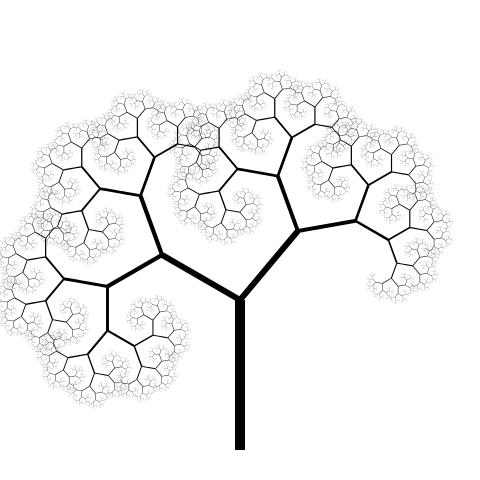
\includegraphics[height=3in]{figs/fractal-tree_60_40.png}
	\caption{a fractal tree with the length ratios of 0.7 and 0.65 and angles of 60 and 40 for left and right branches, respectively.}
	\label{fractal_tree2}
\end{figure}

\subsubsection*{(d)}
\begin{figure}[hb]
	\centering
	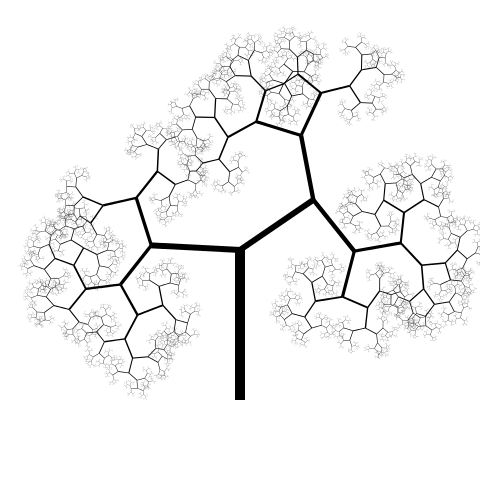
\includegraphics[height=3in]{figs/fractal-tree_rand1.png}
	\caption{a random fractal tree.}
	\label{fractal_tree_rand}
\end{figure}

\begin{figure}[hb]
	\centering
	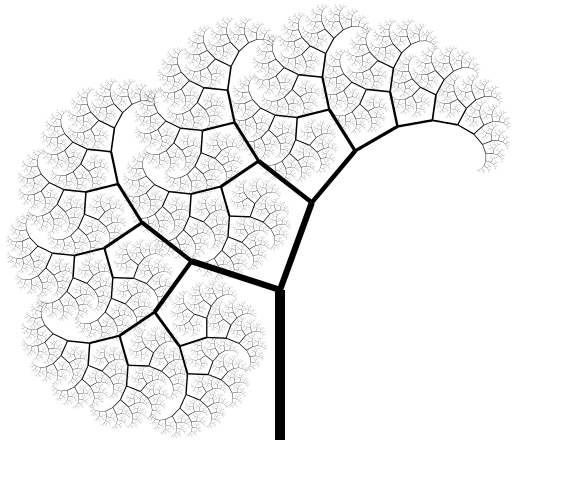
\includegraphics[height=3in]{figs/fractal-tree_interesting.png}
	\caption{a fractal tree with the length ratios of 0.675 and 0.725 and angles of 72 and 20 for left and right branches, respectively}
	\label{fractal_tree_interesting}
\end{figure}

Fig.\ref{fractal_tree_rand} shows a fractal tree which takes a random value $x \in [0.55, 0.8]$ for branching ratio and degree $\theta \in [\frac{\pi}{6}, \frac{\pi}{2}]$. Fig.\ref{fractal_tree_interesting} displays a fractal tree with the length ratios of 0.675 and 0.725 and angles of 72 and 20 for left and right branches, respectively.

\end{document}












